\chapter{Gravity}\label{ch:gravity}

\epigraph{ ``Why are things so heavy in the future?  Is there a problem with the Earth's gravitational pull?''}
{{\normalfont ---\ Dr Emmett Brown}, Back to the Future}

\section{Introduction}

Gravity is the first geophysical method introduced in this course, and it serves as the archetype for all potential-field methods that follow. Gravity measurements sense variations in the Earth's gravitational acceleration produced by lateral contrasts in mass density. Unlike geothermics, gravity does not measure a state variable, nor does it involve time dependence or propagation. The gravity field responds instantaneously to the present-day distribution of mass and therefore contains no intrinsic memory of geological history. What gravity offers instead is a direct window into how geometry and density combine to shape an observable field.

From a geophysical perspective, gravity is fundamentally an integrative method. Every mass contrast within the Earth contributes to the measured signal, and the observed gravity anomaly represents the superposition of contributions from structures at all depths and scales. Nearby and shallow sources tend to dominate short-wavelength features, while deeper and more extensive structures control long-wavelength trends. As a result, gravity is exceptionally sensitive to geometry—depth, thickness, lateral extent, and shape—often more so than to the precise value of density itself. Understanding how geometry controls anomaly form is therefore central to gravity interpretation.

Gravity is also the clearest setting in which to confront non-uniqueness. Many different mass distributions can produce indistinguishable gravity anomalies, and no gravity dataset alone can uniquely determine subsurface structure. Interpretation necessarily proceeds by constructing forward models, applying geological constraints, and asking what classes of models are consistent with the observations. Rather than a limitation of the method, this non-uniqueness is a defining feature of potential fields and motivates the careful use of simplified source models, assumptions, and corrections.

In this chapter, gravity is developed as a steady-state potential field governed by Newtonian gravitation and Poisson's equation. We emphasize the principle of superposition, the role of canonical source geometries, and the connection between density variations and Earth structure and composition. Gravity provides the first opportunity in the course to see how simple models, forward calculations, and geological reasoning combine to extract physically meaningful constraints from inherently ambiguous data. These ideas will recur throughout the remaining geophysical methods and form the conceptual foundation for inversion and computational approaches introduced later.

Gravity — Revised Planning Outline
Framing \& motivation

Gravity as the archetypal potential field
What gravity measures and what it does not

Key ideas

Superposition
- Geometry dominance
- Non-uniqueness
- Steady-state behaviour

Physical basis
- Newtonian gravitation
- Potential, field, Poisson's equation

Superposition and building anomalies
- From bodies to geology
- Additivity as the organizing principle

Canonical source models
- Sphere
- Infinite cylinder (2D)
- Infinite slab
- Point mass (conceptual)

Density of Earth materials
- Minerals → rocks → porosity
- Revisiting mixing laws

Corrections as geological assumptions
- What is removed
- What is assumed

Forward modeling paradigms
- Talwani (2D)
- Pixel / voxel models
- Vertical columns
- Equivalent sources

Non-uniqueness and interpretation
- Equivalence
- Limits of gravity alone

Looking Ahead
- Magnetics
- Inversion
- Isostasy (as separate chapter)

\ntextbox{Key Concepts}{
\begin{itemize}
    \item \textbf{Gravity measures a force field produced by mass contrasts, not a state variable.}

    Gravity observations reflect the present-day distribution of mass density and contain no intrinsic time dependence or memory of geologoical history.

    \textit{How does this distinguish gravity from methods that measure state variables (e.g., temperature) or time-dependent signals (e.g., waves)?}

    \item \textbf{Gravity anomalies arise through superposition of contributions from all mass contrasts.}

    Every density contrast within the Earth contributes additively to the observed field, making superposition the organizing principle for both interpretation and modeling.

    \textit{How can complex geological structures be decomposed into simpler components for forward modeling?}

    \item \textbf{Geometry controls gravity signals more strongly than precise density values.}

    Depth, thickness, lateral extent, and shape exert first-order control on anomaly amplitude and wavelength, often dominating over uncertainty in density itself.

    \textit{Which geometric parameters most strongly influence the observable gravity field?}

    \item \textbf{Gravity is a steady-state, instantaneous field with no intrinsic memory.}

    The gravity field responds immediately to changes in mass distribution and contains no information about the timing or history of geological processes.

    \textit{What kinds of geological questions are therefore inaccessible to gravity alone?}

    \item \textbf{Gravity is inherently non-unique.}

    Many different mass distributions can produce indistinguishable gravity anomalies, and gravity data alone cannot uniquely determine subsurface structure.

    \textit{What additional geological or geophysical constraints are required to reduce ambiguity?}

    \item \textbf{Canonical source models are deliberate abstractions that build intuition and constrain interpretation.}

    Simple bodies such as spheres, cylinders, and slabs are not realistic representations of geology, but they reveal scaling behavior, depth sensitivity, and bounding limits on plausible structures when the appropriate abstraction is chosen.

    \textit{How can an oversimplified model still provide meaningful constraints on real Earth structure?}

    \item \textbf{Analytic gravity models provide benchmarks for numerical forward and inverse methods.}

    Numerical codes should be able to reproduce analytic solutions within expected tolerance; failure to do so indicates problems with implementation rather than geology.

    \textit{Why are benchmark tests essential before interpreting results from complex numerical models?}

    \item \textbf{Density variations reflect Earth structure and composition.}

    Variations in mineralogy, lithology, porosity, pressure, and temperature give rise to density contrasts that underpin gravity anomalies.

    \textit{How do compositional and structural factors translate into observable density contrasts?}

    \item \textbf{Gravity corrections encode geological assumptions.}

    Latitude, free-air, Bouguer, terrain, and related corrections are not purely technical adjustments but reflect specific assumptions about reference structures and mass distributions.

    \textit{How do different correction choices change the geological meaning of a gravity anomaly?}

    \item \textbf{Gravity interpretation relies on forward modeling rather than direct inversion.}

    Interpretation proceeds by proposing models, computing their gravity response, and assessing consistency with observations rather than by recovering a unique solution.

    \textit{How does forward modeling shape the way gravity data are interpreted compared to imaging methods?}
\end{itemize}
}{core}
% \begin{itemize}
%     \item How do the force of gravity, the gravitational attraction, and the
%     gravitational potential relate to one another? 

%     \item How do we determine the gravitational attraction due to an object?

%     \item What corrections must be applied to gravity data?

%     \item What gives rise to variations in density?
% \end{itemize}

\section{Mathematical symbols and units}
\begin{table}[hbt]
    \caption{Definitions of symbols.\vspace{2pt}}
    \label{tab:gravsym}
    \begin{tabular*}{\textwidth}{@{}cll@{}}
        \toprule
        Symbol &
        Quantity &
        SI Unit \\
        \midrule
        $x$, $y$, $z$   & distance                      & meter, m \\
        $r$             & radius                        & meter, m \\
        $m$             & mass                          & kilogram, kg \\
        $V$             & volume                        & m$^{3}$ \\
        $\rho$          & mass density                  & kg~m$^{-3}$ \\
        $\vb{F}$      & force                         & newton, N = kg~m~s$^{-2}$ \\
        $U$             & gravitational potential       & joule, J = N~m \\
        $\vb{g}$      & gravitational acceleration    & m~s$^{-2}$ \\
        $G$             & gravitational constant        & $6.6725985 \times
            10^{-11}$m$^{3}$~kg$^{-1}$~s$^{-2}$ \\
        %$\lambda$       & wavelength                    & m \\
        %$k$             & wavenumber ($k = 2\pi \lambda^{-1}$)
        %    & radians m$^{-1}$ \\
        \bottomrule
    \end{tabular*}
\end{table}

The standard SI units of gravitational acceleration are m~s$^{-2}$, where 1~m~s$^{-2}$ is equivalent to 10$^2$~cm~s$^{-2}$ in the cgs system.  We also call the cgs unit the Gal (sometimes gal, after Galileo).  For geophysics, the changes that we seek are often much smaller than a Gal.  So we commonly use the mGal ({\it milli}-Gal, 10$^{-5}$~m~s$^{-2}$) and $\mu$Gal ({\it micro}-Gal, 10$^{-8}$~m~s$^{-2}$).


\section{Theory}
In this section, we will cover the derivation of the gravitational attraction from the gravitational potential due to a uniform distribution of mass.  The goal is to develop a relationship that we can use to model gravity for a known geometry.  While we want ultimately want gravity, it is easier to work with the scalar potential than gravity, a vector quantity.  So the general procedure is to find the potential using superposition of small volumes of equal density and add them up---integrate over volume---and then find the gradient in the potential---take the derivative.

The Newtonian law of universal gravitation state that the magnitude of force due to gravity is proportional to the product of the masses and the inverse square of the distance between them,
\begin{equation}
    \vb{F} = G \frac{m m_0}{r^2} \vu{r}.
\end{equation}
A $\vu{r}$ is added to indicate that the force acts in a line defined by the centers of the two masses.  In addition, we must add a constant, $G$, to make the units work out properly since Newton's formulation is actually a proportionality.  The distance between the two masses, $r$, is determined by their relative positions in space.  If we place one mass at $P$ located at $(x,y,z)$ and a second at $P'$ located at $(x',y',z')$, the distance between the two masses is given by the Pythagorean theorem:
\begin{equation}
    r = [(x - x')^2 + (y - y')^2 + (z - z')^2]^{1/2}
\end{equation}
(Fig.~\ref{fig:twomass}).  The direction of the line between the centers is determined by the differences between the components,
\begin{equation}
    \vu{r} = \frac{1}{r}[(x - x')\vu{x} + (y - y')\vu{y} + (z -
    z')\vu{z}] .
\end{equation}
In order to make $\vu{r}$ a unit vector, we must divide by $r$.  By our definition above, we have defined the origin centered about $P'$.
\begin{figure}[hbt]
    \centering
    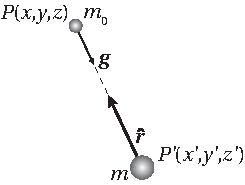
\includegraphics[]{gravity/figures/two_masses2.pdf}
    \caption{Two masses, one of interest $m$ located at $P'$ and the second a test mass, $m_0$, located at our point of observation $P$.  The unit vector is defined outwards from the center of mass, $m$, while the gravitational attraction, $\vb{g}$, at point $P$ due to $m$ is positive towards the center of mass $m$.}
    \label{fig:twomass}
\end{figure}

Above, we have described the relationship between masses and the gravitational attraction.  How can we use this relationship to investigate Earth?  As it stands, it is difficult from just this relationship since it depends on two masses: the mass of interest, $m$, and a mass that we use to measure the force, $m_0$.  But suppose we use multiple instruments to measure mass---Earth is pretty big as you know.  This requires that all $m_0$'s are identical so that the value of the force would be the same for each instrument.  A better approach would be looking for a field which does not require a test mass.

Newton's second law of motion, defines a force as $\vb{F} = m\vb{a}$, where $\vb{a}$ is an acceleration.  If we assume our mass is a test mass
\footnote{We will use the term test mass to indicate a small mass at our point of interest.  A test mass is a place holder within an equation and cancels out of derivations so its exact magnitude is irrelevant.  We will use a similar term to describe poles and charges in future chapters.},
$m_0$, and change the designation of acceleration from $\vb{a}$ to $\vb{g}$, we can write
\begin{equation*}
    \vb{F} = m_0 \vb{g} .
\end{equation*}
Equating the two equations above, we can solve for the acceleration due to
gravity,
\begin{equation}
    \vb{g}(P) = - G \frac{m}{r^2} \vu{r}.
\end{equation}
This result above is {\it fantastic} as it allows us to measure a field that will be the same regardless of the test mass we choose to determine it.  Note: the addition of the minus sign is a matter of convention and indicates that the force points away from our test mass, $m_0$, and in the direction of the mass, $m$.

We also want to get rid of the vector, at least for the moment, as keeping track of vector components can be quite tedious.  Since gravity is a potential field, we can relate the vector gravitational attraction to a scalar gravitational potential, $U$, by
\begin{equation}
    \vb{g}(P) = \grad U(P) .
    \label{eq:gpotential}
\end{equation}
To find the potential from the gravitational attraction,
\begin{align*}
    U(P) &= \int_{\infty}^{P} \vb{g} \cdot \vu{dr}' \\
        &= - G \int_{\infty}^{P} \frac{m}{r'}\vu{r}' \cdot \vu{dr}' \\
        &= -G \Bigg. \frac{m}{r} \Bigg|_\infty^P = G \frac{m}{r} .
\end{align*}

If we wanted to use the equation above to determine the gravitational potential we could do so by employing the principle of superposition,
\begin{equation*}
    U = G \sum_i \frac{m_i}{r_i} .
\end{equation*}
However, can you imagine doing so for an object the the size of Earth?  Even a tiny crystal has so many individual atoms (point masses) that it would be impractical to compute $\vb{g}$ from so many sources.  But there is another, simpler way to employ the principle of superposition assuming the distribution of masses is relatively constant throughout the medium (Fig.~\ref{fig:massdensity}).  We can express this mass distribution as a mass density, $\rho$, in terms of the elemental mass, $\dd{m}$, per elemental volume, $\dd{v}$,
\begin{equation*}
    \dd{m} = \rho \, \dd{v} .
\end{equation*}
Inputting this relationship into the gravitational potential, we find
\begin{equation}
    U(P) = G \int_V \frac{\rho(P')}{r}\, \dd{v} .
    \label{eq:gpot}
\end{equation}
Once we estimate the potential, we simply take the gradient to determine the gravitational attraction as indicated by Eq.~\ref{eq:gpotential},
\begin{equation*}
    \vb{g}(P) = - G \int_V \frac{\rho(P')}{r^2} \vu{r}\, \dd{v} .
\end{equation*}
Assuming mass is constant throughout the body, we can rewrite the above result as
\begin{equation}
    \vb{g}(P) = - G \rho \int_V \frac{\vu{r}}{r^2} \, \dd{v} .
\end{equation}

\begin{figure}[hbt]
    \centering
    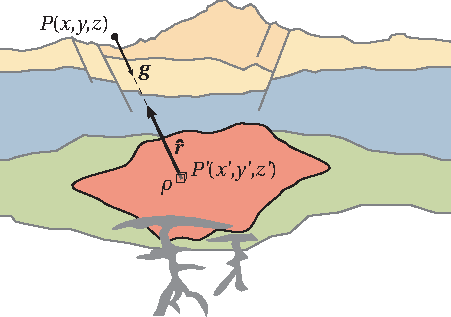
\includegraphics[]{gravity/figures/density.pdf}
    \caption{Instead of adding up each mass, we can describe a body of uniform mass distribution (density, $\rho$) and integrate over volume to determine the gravitational attraction due to the body.}
    \label{fig:massdensity}
\end{figure}

This result provides us with a simpler way to determine the gravitational attraction.  First determine $U$, then differentiate to find $\vb{g}$.

Traditionally gravimeters only measured the vertical component of gravity $g_z$, which was referenced to the geoid (local horizontal as measured by a spirit level).  This method is still the most commonly applied for exploration; hence, we only need to take the vertical derivative of the potential (i.e., $g_z = -\pdv{U}{z}$) for many applications.  The vertical component is given by
\begin{align}
    g_z &= - G \rho \int_z\int_y\int_x \frac{(z - z')}{r^3}\, \dd{x}\,\dd{y}\,\dd{z} &&
    \text{Cartesian} \\
    &= - G \rho \int_z\int_r\int_\phi \frac{(z - z')}{r^2}\, \dd{\phi}\,\dd{r}\,\dd{z} &&
    \text{cylindrical} \\
    &= - G \rho \int_r\int_\theta\int_\phi \sin \theta \cos \theta\,
    \dd{\phi}\,\dd{\theta}\,\dd{r} &&
    \text{spherical},
\end{align}
for each of the commonly used coordinate systems.  These relationships are used to estimate observed gravity from an assumed set of mass distributions.


\section{Gravity Anomalies}
Now that we have a way to determine the potential due to a mass distribution, lets look at some.  Consider a body of uniform density sitting in a half space with a different uniform density.  We will also make an important change in the way we estimate gravity here.  Instead of discussing absolute density, we will describe our bodies of interest in terms of either a mass excess or deficit (i.e. the difference in density between the body of interest and the medium; Fig.~\ref{fig:ds}).  We do this because for the same density contrast, the background gravitational attraction is uniformly increased or decreased by the value of the medium.  However, our measurements are relative which means that we can never be quite sure what the background attraction should be.
\begin{figure}[h]
    \centering
    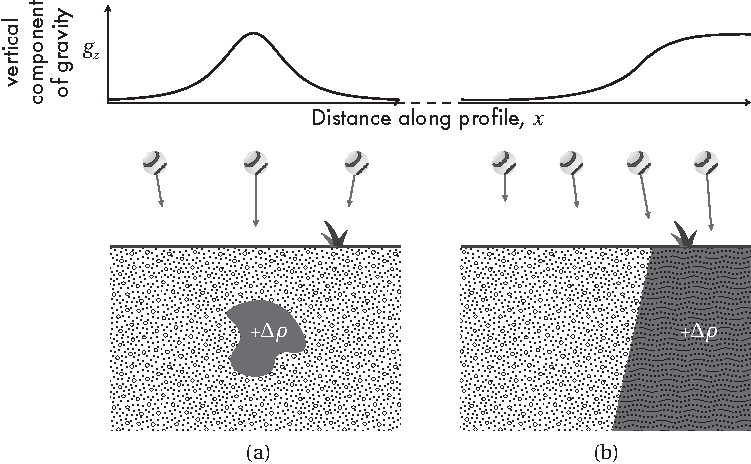
\includegraphics[]{gravity/figures/density_sensitivity.pdf}
    \caption{The gravitational attraction, $\vb{g}$, is changes in response to
    local density variations.}
    \label{fig:ds}
\end{figure}

In the derivations that follow, we will derive the gravity anomalies (or potential) due to several simple geometric objects: a buried sphere; an infinite slab of finite thickness; etc.  You may ask why we do such simple derivations when geologic objects have very complex shapes.  But to first order, geologic structures can approximated by these simple shapes, or perhaps a combination of a few.  For example, diapir shaped intrusions can be approximated as spheres and sedimentary layers or an aquifer can be approximated by the infinite slab. 

\subsection{Spherical Shell}
One of the simplest objects that we can compute the gravitational potential for is a sphere (Figure~\ref{fig:ss}).  While the solution is straightforward and can easily determine the solution without a laborious integration, we will derive the result instead to illustrate how to illustrate the process of computing potential.

Consider a sphere with uniform density, $\rho$, and radius, $a$.  We wish to determine the gravitational attraction due to this sphere at an observation point, $P$, a distance, $R$, from the center of the sphere.  To find the potential, we use Equation~\ref{eq:gpot},
\begin{equation*}
    U(R) = -G \rho \int_V \frac{\dd{v}}{D},
\end{equation*}
where $D$ is the distance to each volume element, $\dd{v}$.  The distance from $P$ to $\dd{v}$ is given by,
\begin{equation*}
    D = (R^2 + r^2 - 2 R r \cos \theta)^{1/2},
\end{equation*} 
where $r$ is the radius of a spherical shell within the sphere.  In spherical coordinates, we can write the each volume element as $\dd{v} = r^2 \sin \theta \,\dd{r} \dd{\theta} \dd{\phi}$.  We want to add up the individual potentials from each volume element.
\begin{figure}
    \centering
    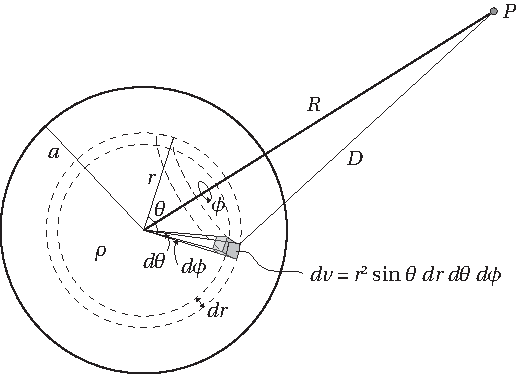
\includegraphics[]{gravity/figures/spherical_shell.pdf}
    \caption{Description of symbols for a spherical shell.}
    \label{fig:ss}
\end{figure}

To do this, we need to integrate over each of the three coordinates:
\begin{align*}
    U(R) &= -G \rho \int_0^a \dd{r} \int_0^\pi \dd{\theta} \int_0^{2\pi} \frac{r^2
        \sin \theta}{(R^2 + r^2 - 2 R r \cos \theta)^{1/2}} \dd{\phi} \\
    &= -2 \pi G \rho \int_0^a \dd{r} \int_0^\pi
        \frac{r^2 \sin \theta}{(R^2 + r^2 - 2 R r \cos \theta)^{1/2}} \dd{\theta} .
\end{align*}
Integrating over $\theta$ is a bit annoying but we can show
\begin{equation*}
    D \,\dd{D} = R r \sin \theta \,\dd{\theta} ,
\end{equation*}
which simplifies our integral considerably,
\begin{align*}
    U(R) &= -2 \pi G \rho \int_0^a \dd{r} \int_{D_{\mathrm{min}} 
        = R - r}^{D_{\mathrm{max}} = R + r} \frac{r}{R} \dd{D} \\
    &= -2 \pi G \rho \int_0^a \frac{r}{R} \Bigg. D \Bigg|_{R - r}^{R + r} \dd{r} \\
    &= -2 \pi G \rho \int_0^a \frac{r}{R} [R + r - (R - r)] \dd{r} \\
    &= -4 \pi G \rho \int_0^a \frac{r^2}{R} \dd{r} .
\end{align*}
Our final step is to then take the integral over $r$,
\begin{align*}
    U(R) &= -\frac{4}{3} \pi G \rho \Bigg. \frac{r^3}{R} \Bigg|_0^a \\
    &= -\frac{4}{3} \pi G \rho \frac{a^3}{R} .
\end{align*}

We will leave the derivation of the gravitational attraction to the problem set.

\subsection{Infinite Slab}
Consider a circular slab of finite extent (we will get to the infinite part later) with a radius of $R$, thickness, $h$, and a uniform density distribution, $\rho$ (Figure~\ref{fig:slab}).  We wish to find the vertical component of gravity, $g_z$, due to this slab at point, $P$, at a distance $b$ above the surface.  Starting with the general gravitational potential, equation \ref{eq:gpot},
\begin{equation*}
    U(P) = -G \rho \int_V \frac{\dd{v}}{D} .
\end{equation*}
We will perform the integration over the volume of the infinite slab in cylindrical coordinates to exploit symmetry and convenience of the system that are more difficult to do in a Cartesian reference frame.
\begin{figure}[bthp]
  \centering
  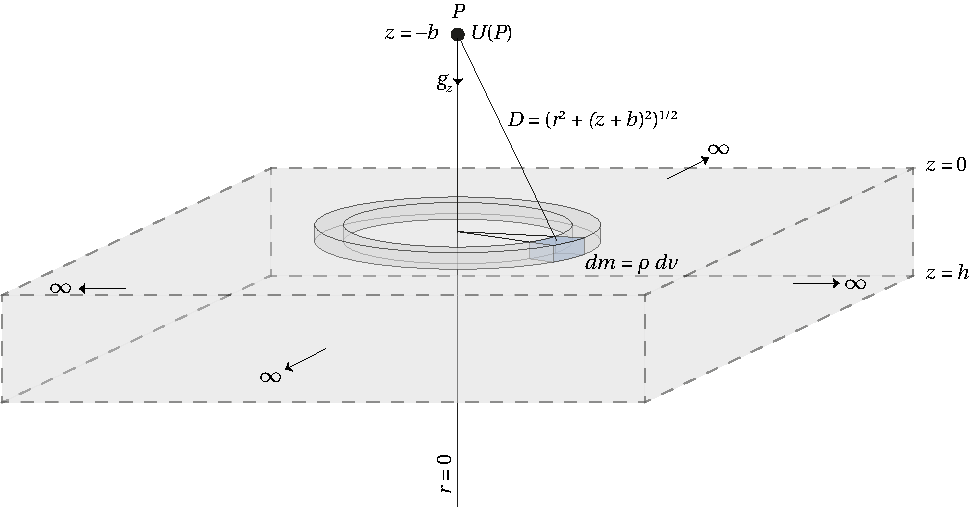
\includegraphics[width=\textwidth]{gravity/figures/infinite_slab.pdf}
  \caption{An infinite slab with thickness, $h$, and density, $\rho$.  Our observation point, $P$, sits a distance $b$ above the surface.  Each infinitesimally small volume, $dv$, has a mass, $dm = \rho dv$.  Note: as is often the case with geophysics, we have defined the $z$-axis as positive down.  Also defining the top of the slab to be at $z=0$ results in a negative value for the height above the surface.}
  \label{fig:slab}
\end{figure}

Sitting at an observation point above the slab, we will integrate over the volume of the slab by integrating infinitesimally small segments around a cylindrical rings and starting from the axis moving away and from the top to the bottom of the slab (Figure~\ref{fig:slab} and \ref{fig:dv}.
\begin{figure}[bthp]
  \centering
  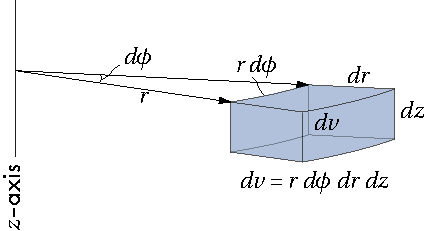
\includegraphics{gravity/figures/volume_element.pdf}
  \caption{A volume element as defined by the cylindrical coordinate system.}
  \label{fig:slab}
\end{figure}
First though, we need to write our potential in cylindrical coordinates.  A volume element in cylindrical coordinates is defined as $\dd{v} = r \dd{\phi} \dd{r} \dd{z}$.  The distance from the observation point to the volume element, $D = (r^2 + (z + b)^2)$.  Hence, the potential in cylindrical coordinates is given by
\begin{equation*}
    U = -G \rho \int_0^h \int_0^R \int_0^{2\pi}
    \frac{r \dd{\phi} \dd{r} \dd{z}}{(r^2 + (z + b)^2)^{1/2}}
\end{equation*}
Note: even though this is an infinite slab, we will perform the integration for a slab of finite radius $R$ and later discuss the implications as $R \to \infty$.  To find the gravitational acceleration, we need to take the gradient of potential.  We are only interested in the vertical component of gravity, so
\begin{equation*}
    \pdv{}{z} U(D) = \pdv{}{z} \left[ -G \rho \int_0^h \int_0^R \int_0^{2\pi}
    \frac{r \dd{\phi} \dd{r} \dd{z}}{(r^2 + (z + b)^2)^{1/2}} \right]
\end{equation*}
Since only the denominator of the fraction within the integral has a z-term, all other components can be assumed constants during integration, i.e.,
\begin{equation*}
    g_z = \pdv{}{z} U = -G \rho \int_0^h \int_0^R \int_0^{2\pi} r \dd{\phi}
    \dd{r} \dd{z} \pdv{}{z} \frac{1}{(r^2 + (z + b)^2)^{1/2}} .
\end{equation*}

Evaluating the derivative, we find
\begin{align*}
    \pdv{}{z} \frac{1}{(r^2 + (z + b)^2)^{1/2}}
    &= -\frac{1}{2} 2 (z + b) \frac{1}{(r^2 + (z + b)^2)^{3/2}} \\
    &= -\frac{(z + b)}{(r^2 + (z + b)^2)^{3/2}} .
\end{align*}
Inserting this result back into the vertical gravitational acceleration above,
\begin{equation*}
    g_z = -G \rho \int_0^h \int_0^R \int_0^{2\pi} 
    \frac{(x + b) r \dd{\phi} \dd{r} \dd{z}}{(r^2 + (z + b)^2)^{3/2}} .
\end{equation*}
Integrating around the cylindrical ring (over $\phi$) is easy since there are no
$\phi$'s in our expression and can all be assume constant.  The integral we are
performing is
\begin{align*}
    \int_0^{2\pi} \dd{\phi} &= \bigl. \phi \bigr|_0^{2\pi} \\
    &= 2\pi - 0 = 2\pi .
\end{align*}
Inserting this result into our equation above,
\begin{equation*}
    g_z = -2 \pi G \rho \int_0^h \int_0^R
    \frac{(x + b) r \dd{r} \dd{z}}{(r^2 + (z + b)^2)^{3/2}} .
\end{equation*}
Next, we perform the integration over $r$ from the axis out to the edge of the
slab,
\begin{align*}
    \int_0^R \frac{(x + b) r \dd{r}}{(r^2 + (z + b)^2)^{3/2}} 
    &= \left.  \frac{-(z + b)}{(r^2 + (z + b)^2)^{1/2}} \right|_0^R. \\
    &= -\frac{(z + b)}{(R^2 + (z + b)^2)^{1/2}} + \frac{(z + b)}{((z + b)^2)^{1/2}} \\
    &= -\frac{(z + b)}{(R^2 + (z + b)^2)^{1/2}} + \frac{(z + b)}{((z + b)} \\
    &= -\frac{(z + b)}{(R^2 + (z + b)^2)^{1/2}} + 1 .
\end{align*}
Inserting this result into $g_z$, we find,
\begin{equation*}
    g_z = -2 \pi G \rho \int_0^h \int_0^R
    \left[ 1 - \frac{(z + b)}{(R^2 + (z + b)^2)^{1/2}} \right] \dd{z} .
\end{equation*}
We need to perform one last to integration to derive the gravitation due to a slab with finite extent,
\begin{align*}
    \int_0^h \left[ 1 - \frac{(z + b)}{(R^2 + (z + b)^2)^{1/2}} \right] \dd{z} 
    &= \int_0^h dz - \int_0^h \frac{(z + b)}{(R^2 + (z + b)^2)^{1/2}} \dd{z} \\
    &= \bigl. z \bigr|_0^h + \bigl. (R^2 + (z + b)^2)^{1/2} \bigr|_0^h \\
    &= h + (R^2 + (h + b)^2)^{1/2} - (R^2 + b^2)^{1/2} .
\end{align*}
Inserting this result, we arrive at
\begin{equation}
    g_z = -2 \pi G \rho [h + (R^2 + (h + b)^2)^{1/2} - (R^2 + b^2)^{1/2}] .
\end{equation}

Now that we have an expression for a slab with finite extent, let us consider what happens as $R \to \infty$.  As $R \to \infty$, the $R^2$ term dominates over the other terms, i.e., $R >> b^2$ and $R >>(h + b)^2$ terms.  Hence, these terms can be considered negligible, resulting in the approximation,
\begin{equation*}
    g_z = -2 \pi G \rho [h + R - R] .
\end{equation*}
as $R \to \infty$.  Simplifying,
\begin{equation}
    g_z = -2 \pi G \rho h .
\end{equation}

The above result for an infinite slab is also known as the Bouguer slab approximation.  Note the result does not depend on the actual height above the slab.  We can use this approximation whenever the extent of the slab is much much greater than our height above it.


\section{Measuring Gravity}
Gravity is perhaps the second most accurate measurement that we can make after frequency (time).  Gravity measurements can be measured to an accuracy of 1 part per billion (1~$\mu$Gal).
\begin{framed}
\noindent {\bf Aside:} Lets put this 1 ppb precision in perspective.  If you had a cubic meter of sand (1~m$^{3}$ = (1000~mm)$^{3}$ = 10$^{9}$~mm$^{3}$, 1 ppb would be the number of grains contained in 10$^{-9} \times 10^{9}$~mm$^{3}$ or 1~mm$^{3}$.  A grain of sand is about 0.2 mm in size so in 1~mm$^{3}$ there are
\begin{equation*}
    \left[ (1 \mbox{ mm}) \times \frac{1}{(0.2 \mbox{ mm/grain})} \right]^{3} =
    25 \mbox{ grains of sand}. \nonumber
\end{equation*}
So if we were to put a cubic meter of sand on a scale, we could measure the
addition of 25 grains to its mass.
\\

What is the mass of 25 grains of sand? (Hint: see table~\ref{tab-density}).
\end{framed}

\subsection{Absolute gravity}
Absolute gravity involves directly measuring the gravitational attraction.  However, this is rarely done because of the expense.  Although some large surveys may make a few absolute gravity measurements that are then used as permanent base stations.

\subsubsection{Pendulum}
Prior to the 1960's gravity was measured using pendulums.  

The period, $\tau$, of a pendulum is given by
\begin{equation}
    \tau = 2\pi \left( \frac{L}{g} \right)^{1/2},
\end{equation}
where $L$ is the length of the pendulum and $g$ is the acceleration due to gravity.  So the gravity can be found by knowing only the length of the pendulum and measuring the period of oscillation,
\begin{equation}
    g = L \left( \frac{2 \pi}{\tau} \right)^{2}.
\end{equation}
To reduce uncertainty, the length of the pendulum was typically quite long and the experiment run for many hours.

\subsubsection{Weight drop}
More modern methods for measuring gravity use mass drop systems.

The distance traveled, $z$, by a test mass under gravity with no initial velocity is proportional to the time, $t$,
\begin{equation}
    z = \frac{1}{2}gt^{2}.
\end{equation}
Thus by measuring the distance the mass has fallen at several discrete time intervals we can estimate $g$,
\begin{equation}
    g = \frac{2x}{t^2}.
\end{equation}

\subsection{Relative gravity}
Most studies use relative gravity because it is cheap and relatively fast to cover large areas.  For a land-based observation, an experienced operator can make a measurement in about two minutes including setup, although for micro-gravity surveys a time series measurement allows for significantly more accurate measurements while also allowing for a more rigorous observational uncertainty.

\subsection{Gradiometer}
There is another type of gravity meter (the gravity gradiometer) that is rarely discussed in textbooks, largely because it is relatively new and not widely used at present.  Although I expect this to change as the instruments become more common and processing methods improve.

In relative gravimetry we are only concerned with the vertical component of gravity, $g_{z}$.  Gravity gradiometry explores derivatives in the gravity field.  For example, the vertical gravity gradient is given by $\Gamma_{zz} = \frac{\partial g_{z}}{\partial z}$.  Gradiometry surveys are almost often airborne experiments which also make them expensive to collect.

An advantage of gradiometry is that it is far more sensitive to shallow density variations making it an ideal for investigating exploration targets.  Because it is a derivative method, it is also more susceptible to noise in the data than standard methods.


\section{Gravity Corrections}
We are often not interested in absolute gravity but relative changes that reflect lithology and structure.  Therefore, the first step in any exploration gravity study is to reduce the observations to a common datum (the reference ellipsoid).  The gravity variations we observe comes from a number of different influences \citep{Blakely1995},
\begin{eqnarray*}
    \mbox{observed gravity} 
    & = & \mbox{ attraction of the reference ellipsoid (latitude)} \\
    & & + \mbox{ time-dependent variations (tidal)} \\
    & & + \mbox{ effect of moving platform (E{\"o}tv{\"o}s)} \\
    & & + \mbox{ effect of elevation above sea level (free-air)} \\
    & & + \mbox{ effect of `normal' mass above sea level (Bouguer and terrain)} \\
    & & + \mbox{ effect of masses that support topographic loads (isostatic)} \\
    & & + \mbox{ effect of crust and upper mantle density variations (`geology')}.
\end{eqnarray*}
Hence we subtract off these other contributions to arrive at a gravity `anomaly'.  Fig.~\ref{fig:gcorr} illustrates how these corrections physically combine to build to derive the gravity anomaly.
\begin{figure}
    \centering
    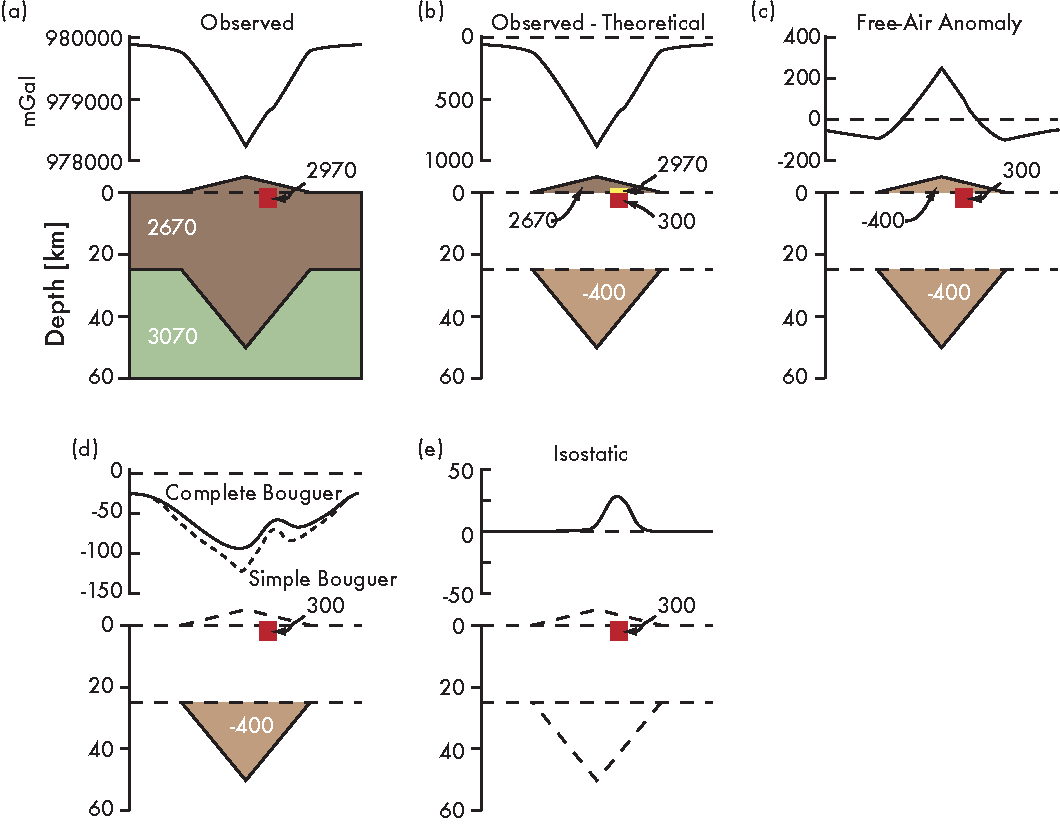
\includegraphics[width=\textwidth]{gravity/figures/gravity_corrections.pdf}
    \caption{Gravity corrections. (a) Observed gravity for a single density crust with a mountain root and an upper crustal anomaly. (b) Removing theoretical gravity (latitude correction). (c) Free-air corrected anomaly. (d) Bouguer correction (simple, slab; complete, slab + topography). (e) Isostatic corrected gravity.}
    \label{fig:gcorr}
\end{figure}

\subsubsection{Instrument Drift}
With time, properties of the gravity meter change ever so slightly resulting in slow change (drift) in readings.  This drift may be due to non-elastic stretching of the spring and mechanical dislocations in the spring at a molecular level among other things.  Essentially these are things that are difficult to impossible to account for directly.  Instrument drift can be non-linear and need not be continuous.  This makes accounting for drift somewhat challenging.  However, the standard method is to take multiple readings at a base station throughout the day (Fig.~\ref{fig:drift}).  By comparing measurements at the base throughout the day a linear-piecewise or low-order polynomial drift curve is developed which is then removed from the data by interpolation.
\begin{figure}[hbt]
    \centering
    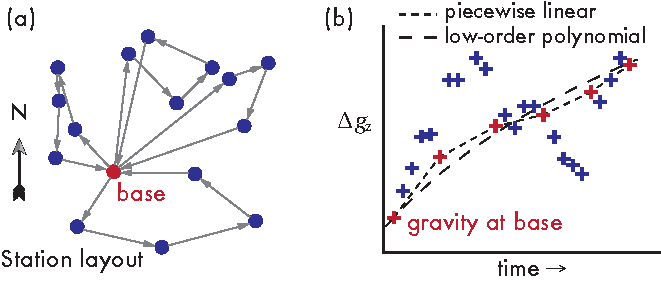
\includegraphics[]{gravity/figures/g_drift.pdf}
    \caption{An illustration of instrument drift for a collection of gravity observations made over a period of time.  (a) Site locations and observational circuits; note the multiple return trips to the base station.  (b) If there is no drift, the change in base station observations should be within observational uncertainty.  The variation throughout the day requires a drift correction, often executed with a low-order polynomial or piecewise linear function.}
    \label{fig:drift}
\end{figure}

\subsubsection{Latitude}
The rotation of Earth not only flattens its shape into a slight ellipsoid but also imparts a slight centrifugal force.  It is a bit like being pushed to the outside of a car when it makes a turn.  This centrifugal force distorts gravity field and is zero at the poles and maximum at the equator.  The latitude correction accounts for the shape and rotation of this ellipsoid and is also called the theoretical gravity.  For a derivation of the centrifugal force see
\citet{Blakely1995}.
\begin{figure}[hbt]
    \centering
    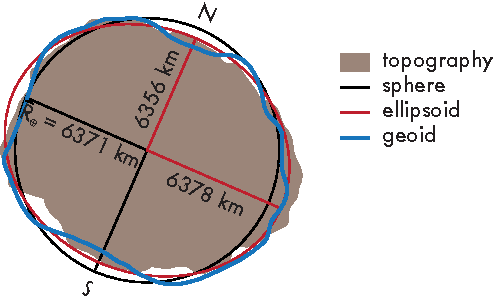
\includegraphics[]{gravity/figures/g_lat.pdf}
    \caption{The shape of Earth deviates from a sphere.  To first order, the shape is an ellipse.  The geoid is an equipotential surface of Earth.}
    \label{fig:latitude}
\end{figure}

Sometimes the latitude correction is handled by using gravity from a local absolute gravity measurement.

The theoretical gravity can be computed using the Somigliana equation,
\begin{equation}
    g_{\lambda} = g_{e} \left( 
    \frac{1 + k \sin^{2} \lambda}{(1 - e^{2} \sin^{2} \lambda)^{1/2}} \right),
\end{equation}
where $g_{e}$ is the equatorial acceleration of the spheroid, $k$ and $e$ are empirical constants.  The Geodetic Reference System 1980 included in the World Geodetic System 1984 (WGS-84), a commonly used datum, the correction is given by
\begin{equation}
    g_{\lambda} = 978032.67714
    \frac{1 + 0.00193185138639 \sin^{2} \lambda}
    {1 - 0.00669437999013^2 \sin^{2} \lambda} \mbox{ $[$mGal$]$}.
\end{equation}
(Better be using double precision numbers in computer codes!)

Sometimes this correction is handled by using observed gravity from a local absolute gravity measurement.

\subsubsection{E{\"o}tv{\"o}s}
When towing a gravity instrument behind a ship, driving in a vehicle, flying in an airplane, or orbiting in a satellite, a correction must be applied for the accelerations imparted by motion.  This correction is unnecessary for the typical land based gravity survey.

For a ship and airplane, the E{\"o}tv{\"o}s correction is given by
\begin{equation}
    g_{E} = 4.051 v \cos \lambda \sin \alpha + 0.001211 v^{2} \mbox{ $[$mGal$]$},
\end{equation}
where $v$ is the speed of travel in km~hr$^{-1}$, $\lambda$ is the latitude w.r.t.\ true north, and $\alpha$ is the heading.

\subsubsection{Tides}
The gravitational pull of the Moon and the Sun distort the shape of the solid Earth.  Hence throughout the day, the distance from a point at the surface to the gravitational center of the Earth changes.  Tides are removed by using precisely calculated tables or mathematical approximations for the location on the Earth and time of day.

\subsubsection{Free-air}
The further one is from the center of the Earth, the lower the gravitational attraction.  The free air correction accounts for the height above sea-level.  This is generally the last correction applied to marine data as there is no elevation above sea-level.

The free-air correction is given by
\begin{equation}
    g_{\mathrm{\it fa}} = 0.3086 h \mbox{ $[$mGal$]$},
\end{equation}
where $h$ is the height above the datum.

\begin{framed}
{\bf Aside:} Although this is called the free-air correction, we do not actually include the density of air, 1.2~kg~m$^{-3}$.  Is the density of air significant enough at 1000~m that we would notice an effect on gravity?

For a Bouguer slab with a density equal to air, the gravitational anomaly is
\begin{equation*}
    2 \pi (6.6725985 \times 10^{-11} \mbox{ m$^{3}$ kg$^{-1}$ s$^{-2}$})
    (1.2 \mbox{ kg m$^{-3}$}) (1000 \mbox{ m}) 
    = 5.0 \times 10^{-7} \mbox{ m s$^{-2}$},
\end{equation*}
\begin{equation*}
    5.0 \times 10^{-7} \mbox{ m s$^{-2}$} 
    \times 10^{8} \mbox{ $\mu$Gal m$^{-1}$ s$^{2}$} = 50 \mbox{ $\mu$Gal}.
\end{equation*}
This should be measurable.  Perhaps we should agree to call this the
free-vacuum calculation instead?
\end{framed}

\subsubsection{Bouguer slab}
Because the theoretical gravity and free-air correction do not incorporate the mass between the observation point and sea-level, we must apply a correction to account for this mass.  This is called the Bouguer correction and involves removing the mass for an infinite slab of height equal to the measurement location.  This resulting anomaly is called the simple Bouguer anomaly.

The Bouguer correction is given by
\begin{equation}
    g_{\mathrm{\it bs}} = 2 \pi G \rho h,
\end{equation}
where $G$ is the gravitational constant, $\rho$ is the density, and $h$ is the height above the datum.

The reduction density for the Bouguer slab correction is almost always assumed to be 2670~kg~m$^{-3}$.  Can you think of a reason this value is chosen?

Assuming the standard reduction density, the Bouguer slab correction is given by
\begin{equation}
    g_{\mathrm{\it bs}} = 0.11194 h \mbox{ $[$mGal$]$}.
\end{equation}

\subsubsection{Terrain}
Local variations in elevation surrounding the station distort the local gravity field, pulling laterally rather than vertically.  The terrain correction accounts for the additional mass above (hills/mountains) the station and missing mass below (valleys).  This correction essentially fixes our incorrect assumption of an infinite slab made in the course of a Bouguer slab correction.  While some of the corrections are simple enough that they can be done by hand---tables exist so that this one may as well---it is best performed by a computer.  This resulting anomaly is called the complex Bouguer anomaly.

\subsubsection{Isostatic}
Local topography may be affected by variations in mass at depth.  Think of mountains like icebergs, only a small percentage of the iceberg sits above the surface.  The height of an iceberg above the water is largely controlled by the amount below.  Likewise, a mountain roots affects its height.  This effect is a long wavelength feature in the gravity and by removing it, in a manner similar to the topographic correction, we can reveal gravity anomalies due to near-surface density variations. Isostasy is discussed further in Chapter~\ref{ch:isostasy}.


\section{Regional residuals}
Typically when utilizing gravity we are looking for `near' surface or `deep' structure.  Changes in observed gravity due to density variations happen over very short distances from near surface structures (short wavelengths) and happen over much longer distances from deep structure (long wavelengths); hence we can exploit this tendency to `filter' gravity.  There are a number of ways in which this residual correction is approached.  The isostatic correction, discussed in an earlier section, is one such method that attempts to reveal the near surface variations.  This section explores a additional common methods for estimating the regional or residual gravity field.  Many of these methods also work for other potential fields such as magnetics and heat flow.

While the isostatic correction has a physical foundation, the other techniques discussed below are purely mathematical meant to exploit the tendency discussed above.

\begin{framed}
\noindent {\bf Aside:} Near surface variations in density can manifest as long wavelength features.  Can you think of a situation where this might happen?  \\

\noindent Deep structures can never produce short wavelength gravity anomalies.
\end{framed}

\subsection{Visual Regression}
Visual regression is just what it sounds like.  In geophysics, we give it a very technically sounding name\ldots the `eyeball filter.'

{\bf Pros:}
\begin{itemize}
    \item Easy to implement.
    \item In a profile, this can more accurately remove regional fields than polynomial representation, although experience is often key to doing this accurately.
\end{itemize}
{\bf Cons:}
\begin{itemize}
    \item Any time you have to say ``it just looks right'' you leave yourself open to biasing the model.
    \item May not uniformly remove deep structure, or may inadvertently remove shallow structure.
    \item Computers are really fast these days and a great many methods are
    easily applied.  The eyeball filter may be good for a quick and dirty analysis in the field or boardroom, but you hate to have to justify in a paper or report that you just drew it.
\end{itemize}

\subsection{Polynomial representation}
Although there is no physical basis---it is purely mathematical---for removal of regional residuals by using low-order polynomials, it is sometimes employed because of its simplicity.  The polynomial surface is given by
\begin{equation}
    g_{\mathrm{poly}}(x,y) = \left( a_{0} + a_{1} x + a_{2} x^2 + \ldots \right)
    \left( b_{0} + b_{1} y + b_{2} y^2 + \ldots \right),
\end{equation}
where $a_{i}$'s and $b_{i}$'s are fitting constants.  The constants can be
determined using a least squares method.

{\bf Pros:}
\begin{itemize} %\setlength{\itemsep}{-5pt}
    \item Easy to implement.
    \item Easy to test higher, or lower orders.
\end{itemize}
{\bf Cons:}
\begin{itemize}
    \item You may have noticed the rather general statement `low-order'.  This is because the polynomial order is at some level up to the user's
    discretion based on the desired size/depth of target anomalies.

    \item The computed surface passes through the mean gravity and therefore the sign of the anomalies have little significance.

    \item Because the model is mathematical and not physical it may poorly fit the regional field.
\end{itemize}

\subsection{Fourier-domain filtering}
Filtering is a common operation in geophysical techniques and Fourier transforms and their inverse are an essential part of this process.  (See the supplemental notes on Fourier transforms.)  Filtering is a common way to examine only the wavelengths of interest within a signal (continuous or discrete).

By in large, the discrete Fourier transform is used most often in geophysics as we collect discretely sampled data.  A Fourier transform is performed on the data (or interpolated grid) in order to generate a set of amplitude and phases of periodic functions (sines and cosines) which describe the data.

Filtering is conducted by convolving the filter function with the gravity surface.  This is typically non-trivial in the spatial domain, but is made much simpler in the Fourier domain where it is simply a multiplication of the Fourier transform of each function.

Suppose we wish to filter the gravity map, $g(x,y)$, using a filter $f(x,y)$, then the filtered gravity $g_{f}(x,y)$ is given by
\begin{equation}
    g_f(x,y) = g(x,y) * f(x,y) \longleftrightarrow G(k_{x},k_{y}) F(k_{x},k_{y}),
\end{equation}
where $G$ and $F$ are the Fourier transforms of $g$ and $f$, respectively.  The mathematical symbol for convolution is $*$.  The spatial frequencies (wavenumbers) are expressed in terms of the spatial wavelengths $k_{x} = 2\pi \lambda_{x}^{-1}$ and $k_{y} = 2\pi \lambda_{y}^{-1}$.  To restore a gravity map, we simply apply the inverse discrete Fourier transform.  Filters are generally developed in the Fourier domain so that they have desirable properties such as removing wavelengths outside the range of interest and produce as few artifacts in the filtered result as possible.

{\bf Pros:}
\begin{itemize}
    \item Can be used to filter regional (low pass) or residual fields (high pass).
    \item Wavelengths can be specifically targeted.
    \item Fourier-domain filtering is a subject area with rich literature.  Numerous filters have been designed to reduce the addition of artifacts in the filtered field.
    \item No need to subtract off a regional field to arrive at a residual.
\end{itemize}
{\bf Cons:}
\begin{itemize}
    \item Filter design is important, a poorly designed filter can add artifacts to the data.
    \item Sparse data are subject to possible aliasing and therefore erroneous interpretation.  A serious issue with aliasing is that you will never know you have done it.
\end{itemize}

\begin{framed}
\noindent {\bf Aside:}  For a digital signal---this includes discretely sampled gravity data---the highest frequency that can be represented by within the signal is the Nyquist frequency, $f_{Ny} = (2 \Delta t)^{-1}$, where $f$ is the frequency and $t$ is time.  For spatial cases such as gravity observations this can be written, $k_{Ny} = (2 \Delta z)^{-1}$.  This really means that the absolute minimum number of times a signal must be sampled to retain the wavelength in the data is twice per cycle.  However, in practice a minimum of four times is required when noise exists (which is always).  Even at four samples per cycle there is a special case where a wavelength can be lost from the signal.  Can you think when that might occur?

When a signal is under-sampled (i.e.\ below the Nyquist frequency) we call this {\it aliasing}.  The signal is distorted from the true signal and often not in an obvious and detectable way.  To make matters worse the aliased frequencies appear as low frequencies in the data that do not really exist.

As an example, consider the Great Basin of North America where roughly north-south trending mountain ranges are separated by sedimentary basins in a near periodic way.  If one were to collect a single gravity observation within each basin, the geologic structures would be aliased within the data.  The gravity observations in this case would look like a long wavelength negative density anomaly due to the sedimentary basins.  The high density contrasting ranges would be missed from the short wavelength features and would likely appear as a very long wavelength feature.
\end{framed}

\subsection{Continuation}
\subsubsection{Gravitational potential}
Before we discuss continuation, we must first define a quantity called the gravitational potential.  At an observation point $P = (x_{0}, y_{0}, z_{0})$, with test mass $m_{0}$, the gravitational force from a mass, $m$, at point $Q = (x,y,z)$ is given by
\begin{equation}
    \vb{F} = G \frac{m m_{0}}{r^{2}}\vu{r},
\end{equation}
where and $r$ is the distance between points $P$ and $Q$, $r = \left[(x_{0} - x)^2 +
(y_{0} - y)^2 + (z_{0} - z)^2\right]^{1/2}$.  Recalling $F = m_{0} g$, the
gravitational attraction between the two points is given by
\begin{equation}
    \vb{g} = G \frac{m}{r^{2}}\vu{r} = \nabla U,
\end{equation}
where $U$ is the gravitational potential and $\nabla$ is the gradient operator.  Therefore, the potential at point $P$ is given by
\begin{equation}
    U(P) = G\int_{V} \frac{dm}{r}.
\end{equation}
Suppose the mass at $Q$ has a density distribution equal to $\rho(x_{0},y_{0},z_{0})$, then $dm = \rho(x_{0},y_{0},z_{0}) dv$.  Thus the potential can be written
\begin{equation}
    U(P) = G\int_{V} \frac{\rho(Q)}{r} dv.
    \label{eq-gpot}
\end{equation}

\subsubsection{Upward Continuation}
Although upward and downward continuation may be done from any shaped surface to any other shaped surface, it is easiest to do if we constrain ourselves from one level surface to another.  Consider a point $P = (x, y, z_{0} - \Delta z)$ such that $\Delta z$ is a positive value some distance above the surface $z_{0}$.  (Note that we define $\hat{z}$ as positive down---towards the center of the Earth.  This is a common convention in geophysics.)  It can be shown that the upward continued field is given by
\begin{equation}
    U(x,y,z_{0} - \Delta z) = \frac{\Delta z}{2 \pi} 
    \int_{-\infty}^{\infty} \int_{-\infty}^{\infty} 
    \frac{U(x',y',z_{0})} 
    {\left[(x - x')^2 + (y - y')^2 + \Delta z^2 \right]^{3/2}}
    dx' dy',
\end{equation}
where $U(x',y',z_{0})$ is given in Equation~\ref{eq-gpot}.  See \citet{Blakely1995} for a full derivation.

Upward continuation can also be expressed as a Fourier domain technique.  Let us define
\begin{equation}
    \psi_{u} = \frac{\Delta z}{2 \pi} 
    \left[(x - x')^2 + (y - y')^2 + \Delta z^2 \right]^{-3/2},
\end{equation}
which has the Fourier transform
\begin{equation}
    \mcal{F}[\psi_{u}] = e^{-|k|\Delta z}, \mbox{ z > 0}.
\end{equation}

Hence,
\begin{equation}
    \mcal{F}[U_{u}] = \mcal{F}[U]\mcal{F}[\psi_{u}],
\end{equation}
and all that needs to be done to find the upward continued field is to take the inverse Fourier transform.  The upward continued gravity, is then found by $\vb{g_{u}} = \nabla U_{u}$.

{\bf Pros:}
\begin{itemize}
    \item Relatively simple and physically based.
    \item Highlights regional variations.
    \item Allows for merging two datasets collected at different altitudes.  This is important when comparing land to airborne, airborne to airborne, airborne to satellite data. 
\end{itemize}
{\bf Cons:}
\begin{itemize}
    \item Short wavelengths are not completely removed but amplitudes are merely attenuated.  The higher the continued surface, the greater the attenuation.
\end{itemize}

\subsection{Downward Continuation}
Downward continuation is a precarious operation as it is an `un-smoothing' operation.  The downward continuation is expressed as
\begin{equation}
    \mcal{F}[U_{d}] = \mcal{F}[U]\mcal{F}^{-1}[\psi_{u}],
\end{equation}
where $\mcal{F}^{-1}[\psi_{u}]$ is $e^{+|k|z}$.  Since noise in the data are generally uncorrelated---they are short wavelength features---any noise is amplified.

{\bf Pros:}
\begin{itemize}
    \item Relatively simple.
    \item Highlights short wavelength anomalies.
\end{itemize}
{\bf Cons:}
\begin{itemize}
    \item Amplifies noise.
\end{itemize}

%\section{Image processing techniques}

\section{Densities of Earth Materials}
The density of Earth materials vary considerably from $\sim$50~kg~m$^{-3}$ for pumice to $\sim$19400~kg~m$^{-3}$ for native gold.  However, most silicates (bulk of the crust and mantle) fall between 2500 to 3400~Mg~m$^{-3}$.  A table summarizing a number of common/important materials are given in Table~\ref{tab-density}.

The density of rocks are affected by the porosity (amount of void space), and composition of the grains.  Sedimentary rocks tend to be less dense than crystalline rocks.  Igneous rock densities are largely controlled by their silica content (SiO$_{2}$).  The more SiO$_{2}$ the less dense the rock.  Most ores are very dense making gravity a good exploration tool.

Bulk can be predicted from the densities of their individual components using a mixing relationship.  A mixing relationship is essentially an average of which a great number have been devised.  For density a rock with several mineral constituents each with a density $\rho_{i}$ and volume fraction $v_{i}$.  Within a given volume, the mass of each component is $v_{i} \rho_{i}$, then dividing by the total volume then will give us the effective (or bulk) density,
\begin{equation}
    \rho_{bulk} = \frac{\sum_{i=1}^{N} v_{i} \rho_{i}}{\sum_{i=1}^{N} v_{i}}.
\end{equation}
Hence the effective density is just the arithmetic mean of the components.  Note that this works as well when rocks have pore space.  In such a case, the pore space must be included as a constituent, (i.e.,\ $\phi \rho_{\phi}$, where $\phi$ is the porosity and $\rho_{phi}$ is the density of the air, oil, gas, or water, filling the pore space).
\begin{table}
    \begin{threeparttable}
    \caption{Table of rock and mineral densities in \si{kg.m^{-3}}.}
    \label{tab-density}
    \begin{tabular}{@{}lclclc@{}}
        \toprule
        Rock Type &
        Density Range &
        Material Type &
        Density Range & 
        Material Type &
        Density Range \\

        \midrule
        \multicolumn{2}{c}{\it Sediments (wet)} & \multicolumn{2}{c}{\it Oxides} & \multicolumn{2}{c}{\it Sulfates} \\
        soil        & 1200--2400    & hematite      & 4900--5300 & gypsum        & 2200--2600 \\
        clay        & 1630--2600    & magnetite     & 4900--5200 & barite        & 4300--4700 \\
        gravel      & 1700--2400    & ilmenite      & 4300--5000 \\
        sand        & 1700--2300    & rutile        & 4180--4300 & \multicolumn{2}{c}{\it Native Elements} \\
        sandstone   & 1610--2670    & chromite      & 4200--4600 & copper        & 8700 \\
        shale       & 1770--3200    & cuprite       & 5700--6150 & silver        & 10500 \\
        limestone   & 1930--2900    & manganite     & 4200--4400 & gold          & 15600--19400 \\
        dolomite    & 2280--2900    & cassiterite   & 6800--7100 & coal          & 1200--1800 \\
        {}          & {}            & wolframite    & 7100--7500 & graphite      & 1900--2300 \\
        \multicolumn{2}{c}{\it Igneous Rocks} & uraninite     & 8000--9970 \\
        tuff        & 1000--2400    & {}            & {}         & \multicolumn{2}{c}{\it Non-metallic} \\
        rhyolite    & 2350--2700    & \multicolumn{2}{c}{\it Hydroxides} & salt          & 210--2600 \\
        granite     & 2500--2810    & bauxite       & 2300--2550 & ice           & 880--920 \\
        granodiorite & 2670--2790   & {}            & {}         & sea water     & 1010--1050 \\
        andesite    & 2400--2800    & \multicolumn{2}{c}{\it Carbonates} & fluorite      & 3010--3250 \\ 
        diorite     & 2720--2990    & calcite       & 2710 \\
        basalt      & 2700--3300    & aragonite     & 2950 \\
        diabase     & 2500--3200    & dolomite      & 2280--2900 \\
        gabbro      & 2700--3500    & siderite      & 3700--3900 \\
        peridotite  & 3200--3370    & magnesite     & 2900--3120 \\
        pyroxenite  & 3200--3370    \\
        {}          & {}            & \multicolumn{2}{c}{\it Sulfides} \\
        \multicolumn{2}{c}{\it Metamorphic Rocks} & pyrite        & 4900--5200 \\
        graywacke   & 2600--2700    & pyrrhotite    & 4500--4800 \\
        slate       & 2700--2900    & sphalerite    & 3500--4000 \\
        quartzite   & 2500--2700    & chalcopyrite  & 4100--4300 \\
        marble      & 2600--2900    & covellite     & 4600--4800 \\
        schist      & 2390--2900    & chalcocite    & 5500--5800 \\
        amphibolite & 2900--3040    & malachite     & 3900--4030 \\
        gneiss      & 2590--3000    & molybdenite   & 4400--4800 \\
        eclogite    & 3200--3540    & cobaltite     & 5800--6300 \\
        serpentine  & 2400--3100    & stannite      & 4300--4520 \\
        {}          & {}            & galena        & 7400--7600 \\
        {}          & {}            & cinnabar      & 8000--8200 \\
        \bottomrule
    \end{tabular}
    \begin{tablenotes}
        \item After \citet{Telford_etal1990} pg. 16.
    \end{tablenotes}
    \end{threeparttable}
\end{table}

\nocite{Blakely1995}
\nocite{Chapin1998}
\nocite{Grant&West1965}
\nocite{Lowrie1997}
\nocite{Reynolds1997}
\nocite{Telford_etal1990}

\bibliographystyle{elsarticle-harv}
\bibliography{ref}
